\chapter{Aufgabe 4}

\textit{Nach welchen Kriterien sollte ein Informationssicherheitsbeauftragter ausgewählt
werden? Welche Kenntnisse sind erforderlich? Beschreiben Sie die Auswahl eines
geeigneten Mitarbeiters anhand des Organigramms des Beispielunternehmens.}\\

\noindent
Eine selbstverständliche Anforderung an den ISB sollte sein, dass er eine gewisse Expertise und fachliche Affinität für das Thema Informationssicherheit mit sich bringt.
Dabei ist eine ausgewiesene berufliche Qualifikation oder Zertifizierung in dem Bereich sicherlich ein hinreichendes, aber nicht unbedingt ein notwendiges Kriterium: Die Anforderungen bzgl. der beruflichen Qualifikation werden sich i.d.R. nach öffentlicher Stellung und (volks-)wirtschaftlicher Rolle der Institution unterscheiden.
Eine kleine Internetagentur wird hier andere Maßstäbe ansetzen (müssen) als eine öffentliche Behörde oder ein Unternehmenskonzern mit mehreren Standorten.\\

\noindent
\textit{Münch und Schaumüller-Bichl} führen in~\cite[43]{ITS2} verschiedene Qualifikationen auf, auf die bei der Auswahl eines ISB geachtet werden sollte, darunter:

\begin{itemize}
\itemsep0.5em
\item Identifikation mit den Zielsetzungen der Informationssicherheit
\item Kooperations- und Teamfähigkeit
\item Erfahrungen im Projektmanagement
\end{itemize}

Die Autoren gehen \textit{ebd.} auf weitere Fragen ein, die bei der Auswahl eines ISB berücksichtigt werden müssen, bspw. auf Verantwortlichkeiten eines ISB im Tagesgeschäft:
Vorausgesetzt, der ISB übernimmt Aufgaben anderer Fachbereiche, kann eine entsprechende Aufgabenlast dazu führen, dass der ISB sich nicht ausreichend auf wichtige Tätigkeiten im Bereich Informationssicherheit konzentrieren kann.\\
Es werden außerdem mögliche Interessenkonflikte angesprochen, die entstehen können, wenn ein Kandidat bereits stark im \textit{operativen} IT-Bereich involviert ist - hier könnten sinnvolle bzw. notwendige strategische Entscheidungen konträr zu pragmatischen Lösungen stehen und zu Konflikten führen.
Eine gewisse Neutralität des Mitarbeiters muss gefordert sein sowie die Fähigkeit, rational und objektiv Entscheidungen im Sinne der strategischen Ausrichtung der Institution bzgl. der Sicherheitsziele zu treffen - natürlich unter Wahrung der Verhältnismäßigkeit.\\

\begin{figure}
\centering
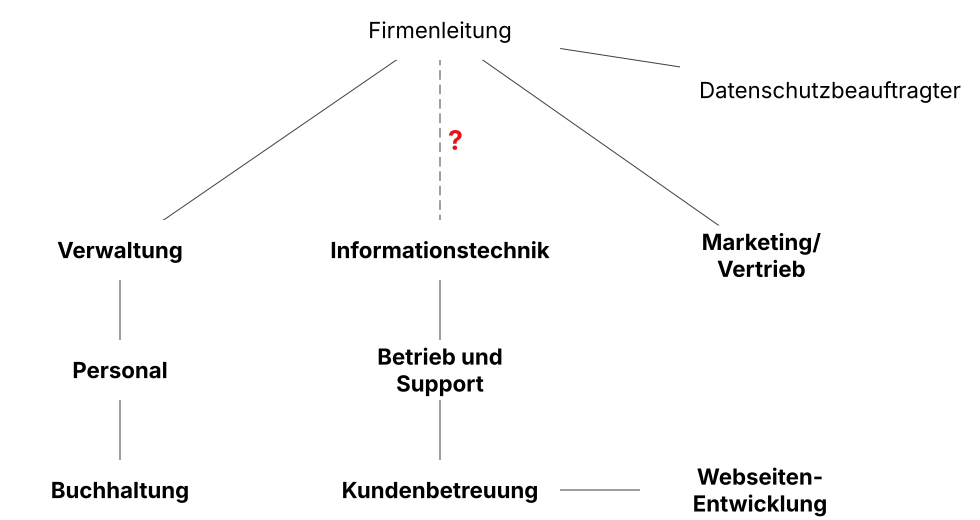
\includegraphics[scale=0.4]{aufgabe 4/img/organigramm.svg}
\caption{Organigramm des Beispielunternehmens. Die in der Aufgabenstellung fehlende Verbindung zwischen Firmenleitung und Informationstechnik ist als gestrichelte Linie dargestellt. (Quelle: in Anlehnung an Abbildung aus Aufgabe 4)}
\label{fig:organigramm}
\end{figure}

\noindent
Das in Abbildung~\ref{fig:organigramm} sinngemäß der Aufgabenstellung dargestellte Organigramm lässt zwei Interpretationen zu:
\begin{enumerate}
\itemsep0.5em
\item Die \textit{fehlende Linie} von \textit{Firmenleitung} zu \textit{Informationstechnik} ist ein Versehen, und die IT ist der Firmenleitung unterstellt (\textit{Fall 1}).
\item Die Verbindung wurde in der Aufgabenstellung bewusst ausgelassen, als Hinweis auf einen externen Dienstleister (\textit{Fall 2}).
\end{enumerate}

\noindent
Beide Fälle werden im Folgenden berücksichtigt.

\begin{itemize}
\itemsep0.5em
\item \textbf{Fall 1}: Personal aus der Verwaltung und dem Marketing wird bei der Auswahl eines ISB nicht weiter berücksichtigt - zwar könnten Mitarbeitende notwendige \textit{Soft Skills} wie \textit{Teamfähigkeit} und \textit{Durchsetzungsvermögen} mitbringen, welche sicherlich dabei unterstützen, Sicherheitsziele zu kommunizieren und Verständnis für notwendige Maßnahmen sowie Bewusstsein für potenzielle Bedrohungen zu schärfen, allerdings wird hier die fachliche Eignung fehlen.\\
Eine Möglichkeit wäre die Auswahl eines Kandidaten aus der IT, wobei hier der o.a. \textit{Interessenkonflikt} zwischen operativem und strategischem ISM bestehen kann.\\
Eine (sehr) gute fachliche Eignung kann sicherlich der Datenschutzbeauftragte mit sich bringen, der der Leitungsebene direkt unterstellt ist und an diese berichtet.
Die fachliche Nähe zwischen \textit{Datenschutz} und \textit{Informationssicherheit} kann hier zu gewissen Synergieeffekten beitragen, allerdings können auch Interessenkonflikte auftreten, wenn Schutzziele verfolgt werden, bei denen durchzusetzende Maßnahmen - wie bspw. die Protokollierung von Nutzerdaten - im Gegensatz zu im Datenschutz verankerten Bestimmungen stehen.\\
Anzumerken ist hier in jedem Fall, dass - je nach Auslastung - ein zusätzlicher Verantwortungsbereich dazu führen kann, dass der ISB die Aufgaben bzgl. ISM nicht zielführend wahrnehmen kann.

\item \textbf{Fall 2}: Die IT ist extern beauftragt.
Obwohl hier aus einem großen Pool externer Dienstleister mit entsprechend hoher Qualifikation und Referenzen ausgewählt werden kann, kann sich eine fehlende Bindung an die Institution sowohl als Vor- als auch als Nachteil erweisen:
Vorteil, weil keine Interessenkonflikte existieren und ISM ``nach Katalog`` zielgerichtet und unabhängig eingeführt werden kann.
Nachteil, weil die Bindung zur Institution fehlt - damit können wichtige wirtschaftliche, politische, soziale und ggf. auch rechtliche Gegebenheiten bei der Bestimmung von Sicherheitszielen nicht oder nur unzureichend berücksichtigt werden. Es besteht die Gefahr, ISM an den eigentlichen Interessen der Institution, ihrer Leitungsebene und den Mitarbeitenden vorbei einzuführen.
In diesem Fall würde wahrscheinlich der bereits existierende Datenschutzbeauftragte der Institution der geeignetste Kandidat sein.
\end{itemize}
